%----------------------------------------------------------------
%
%  File    :  project-design.tex
%
%  Author  :  Keith Andrews, IICM, TU Graz, Austria
% 
%  Created :  27 May 1993
% 
%  Changed :  03 Feb 2017
% 
%----------------------------------------------------------------


\chapter{Changes of the Design}

\label{chap:design}

The design of \textit{rSlidy} has undergone numerous major changes throughout 
our project. A comparison between the old and the new version is given in this 
chapter.

\section{The Status Bar}
The initial version of \textit{rSlidy} was equipped with a permanent status 
bar, as shown in Figure \ref{fig:statusbarOLD}. It has been modified in terms 
of design and functionality. The final appearance of the status bar is shown in 
 Figure \ref{fig:statusbarNEW}. The following individual changes have been made.

\begin{figure}[tp]
	\centering
	
\includegraphics[width = \textwidth]{images/status_bar_old.png}
	
	\caption[Original Status Bar]{
		Design of \textit{rSlidy}'s original status bar.
		\imgcredit{Screenshot taken by the authors of this report.}
	}
	\label{fig:statusbarOLD}
\end{figure}

\begin{figure}[tp]
	\centering
	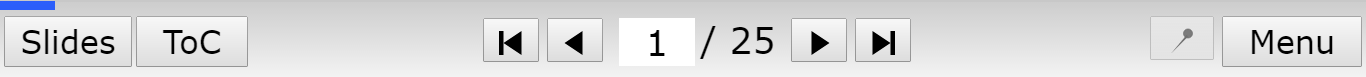
\includegraphics[width = \textwidth]{images/status_bar_new.png}
	
	\caption[Modified Status Bar]{
		Design of \textit{rSlidy}'s modified status bar.
		\imgcredit{Screenshot taken by the authors of this report.}
	}
	\label{fig:statusbarNEW}
\end{figure}


\subsection{Progress Bar}
A simple blue progress bar has been added on top of the status bar. Its purpose 
is to give some visual feedback about the current progress within a 
presentation. Its implementation is fairly simple. The progress bar container's 
width property is changed on each slide change with an animated transition (see 
Listing \ref{list:progressbar}).


\begin{lstlisting}[
language=JavaScript,
label=list:progressbar,
caption={[Progress Bar Width Adaptation] Adapting width of the progress bar 
container for authentic visual feedback
}
]
Rslidy.prototype.showSlide = function (slide_index) {
	// ...
	var progress_bar = document.getElementById("progress-bar");
	progress_bar.style.width =
				'calc(100%*' + (slide_index + 1) / 
this.num_slides + ')';
	// ...
}
\end{lstlisting}

\subsection{Rearrangement / Extension of the Navigation Elements}
We found it simply more intuitive to have the input field for jumping to a 
specific slide in the middle of the forward / backward buttons. Apart from 
this, functionalities to jump to the first and respectively the last slide have 
been added. These two starightforward implementations can be seen in Listing 
\ref{list:firstlastslide}.

\begin{minipage}{\linewidth}
\begin{lstlisting}[
language=JavaScript,
label=list:firstlastslide,
caption={[First / Last Slide Buttons Implementation] Implementation of the 
buttons for jumping to the first / last slide
}
]
document.getElementById("status-bar-nav-button-first")
	.addEventListener('click', function ()
	{
		this.showSlide(0);
	}.bind(this));
document.getElementById("status-bar-nav-button-last")
	.addEventListener('click', function ()
	{
		this.showSlide(this.num_slides - 1);
	}.bind(this));
\end{lstlisting}
\end{minipage}



\subsection{Pin Functionality}
In opposition to the original \textit{rSlidy} status bar, the new one features 
pinning / unpinning. The pinned status bar works the same as the old one. The 
unpinned status bar disappears when not hovering over it. When the mouse is not 
close to the bottom of the document, only the progress bar is visible in the 
unpinned mode. Two subtle triangles have been added to the unpinned status bar 
which are meant to function as little indicators for the actual bar. This 
implementation may not be the most elegant one, because it is relying on the 
title of the button to work properly. Some simple boolean variable which 
describes whether the bar is pinned or not may be a more robust solution. 
Still, this (see Listing \ref{list:pin_unpin}) is what we came up with and it 
works fine as long as the title tag of the pin button in the rslidy.js file is 
either "Pin the status bar" or "Unpin the status bar" (depending on whether the 
user wants the bar to be pinned or not by default).


\begin{minipage}{\linewidth}
\begin{lstlisting}[
language=JavaScript,
label=list:pin_unpin,
caption={[Pin / Unpin Implementation] Implementation of the buttons for pinning 
/ unpinning the status bar 
}
]
Rslidy.prototype.pinToggleClicked = function (close_only) {
	var pin_button = document.getElementById("status-bar-pin-button");
	var status_bar = document.getElementById("status-bar-content");
	var indicator_left = document.getElementById("progress-bar-indicator-left");
	var indicator_right = document.getElementById("progress-bar-indicator-right");

	if (pin_button.title == "Pin the status bar")
	{
		pin_button.title = "Unpin the status bar";
		status_bar.style = "transform: translateY(0);";
		pin_button.style.WebkitTransition = 'opacity 0.3s';
		pin_button.style.MozTransition = 'opacity 0.3s';
		pin_button.style.opacity = 0.5;
		indicator_left.style.visibility = "hidden";
		indicator_right.style.visibility = "hidden";
	}
	else
	{			
		pin_button.title = "Pin the status bar";
		status_bar.removeAttribute('style');
		pin_button.style.opacity = 1;
		indicator_left.style.visibility = "visible";
		indicator_right.style.visibility = "visible";
	}
};
\end{lstlisting}
\end{minipage}

\section{The Menu}
The menu has been modernized and harmonized as seen in a direct comparison of 
Figure \ref{fig:menuOLD} and Figure \ref{fig:menuNEW}. Implementation-wise 
these changes were mostly straightforward:
\begin{itemize}
	\item Partial transparency has been added to the menu. The actual 
document thus slightly shines through the menu.
	\item The corners have been corners in order to get a smoother look in 
general.
	\item Shadow effects have been added to the edges of the menu in order 
to get a very basic 3D-effect.
	\item Harmonization has taken place. All links were exchanged with 
buttons. This means more consistency in the design altogether. 
	\item One more checkbox has been added. It allows the user to switch 
between a version which, as usual, shows the address of a link on hover and a 
version which suppresses that standard function by removing the "href" property 
from all initial links.
\end{itemize}

\begin{figure}[tp]
	\centering
	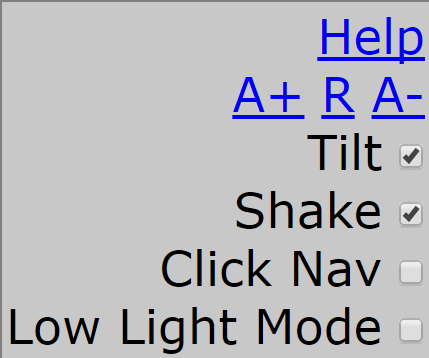
\includegraphics[width = .4\textwidth]{images/menu_old.png}
	
	\caption[Original Menu]{
		Design of \textit{rSlidy}'s original menu.
		\imgcredit{Screenshot taken by the authors of this report.}
	}
	\label{fig:menuOLD}
\end{figure}

\begin{figure}[tp]
	\centering
	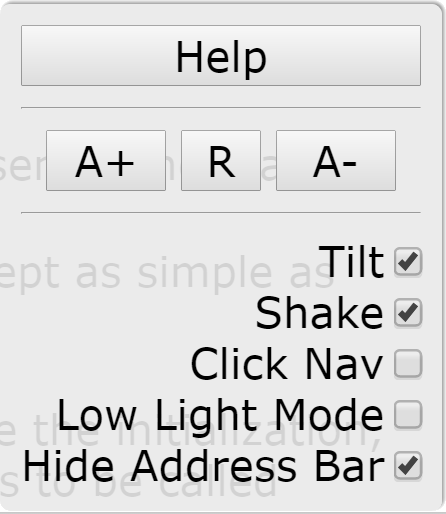
\includegraphics[width = .4\textwidth]{images/menu_new.png}
	
	\caption[Modified Menu]{
		Design of \textit{rSlidy}'s modified menu.
		\imgcredit{Screenshot taken by the authors of this report.}
	}
	\label{fig:menuNEW}
\end{figure}


\subsection{User Set Default Values} % (fold)
\label{sub:user_settings}

By using the menu the user can always change the settings, however there was no 
function previously to define his own defualt settings for each seperate 
presentation. The function was realized through hidden input elements, which in 
initialization trigger the previously built toggle functions. To keep a 
constant structure and preventing mistakes such as forgotten setting in middle 
of code, a container div with id \textit{setupDefaultValues} has to be used 
inside the body to set the defaults. The constraint is only binded on the 
container id and each setting value id. The whole array of settings can be seen 
in code snipplet \ref{list:userSettings}. The whole container can be excluded 
if default values work for the user, otherwise just the wanted changes are 
needed. Between the options please note, that a default font size option was 
added, however it requires the use of em values. The constraint is for correct 
change of font size on button click inside the menu, while the font size reset 
button will used the specified value. This could be solved in multiple ways, 
however em having a good scaling interpratation, it was decided that it 
unneeded.

\begin{minipage}{\linewidth}
\begin{lstlisting}[
language=CSS,
label=list:userSettings,
caption={[User Set Default Values]%
	By adding the container div with id setupDefaultValues, the slideshow 
creator can define, which menu settings or font size should be defualt. The 
values provided in the snipplet are the default values of \textit{rSlidy}. Only 
the desired value changes need to have an hidden input included in the 
container. 
}
]
<div id="setupDefaultValues" class="hidden">
	<!-- //font size should be specified in EM for correct zooming -->
	<input type="hidden" id="default-font-size" value="1em">
	<input type="hidden" id="statusbar-pin-locked" value="false">
	<input type="hidden" id="menu-tilt-used" value="true">
	<input type="hidden" id="menu-shake-used" value="true">
	<input type="hidden" id="menu-click-nav-used" value="false">
	<input type="hidden" id="menu-low-light-mode-used" value="false">
	<input type="hidden" id="menu-hide-address-used" value="false">
</div>
\end{lstlisting}
\end{minipage}

% subsection user_prefered_s (end)

\section{The Help Information}
This information, which can be opened from the menu, used to be a usual alert 
box. Due to the instructor's wish to have no third party libraries included, 
there are two versions of our implementation for the new help popup. The 
initially intended version is based on a library called "sweetalert" 
(\url{https://limonte.github.io/sweetalert2/}). It allows animated popup 
messages with focusing on the actual text. The advantage of this way of 
implementation is the the polished design while having to rely on a third party 
library. The revised version simply opens a new tab to display the help 
message. This does not look as sophisticated as the other version, but still 
works fine and is an independent way of solving the popup problem.


\section{Side Menus} % (fold)
\label{sec:side_menus}

The side menus in \textit{rSlidy} consist of a slide overview and table of 
contents, both shortend in the application as Slides and ToC. In original 
version both menus were fixed in same position on the left side andwere by 
default hidden. By clicking the the menu buttons with their shorten names, the 
user could activate one and switch between both or close them. By overlapping 
different functions and demanding the user to activate either function with 
buttons in same corner of the screen, the workflow is unnaturally limited if 
not broken. Even more on mobile devices.

Therefore the refined version changed the design by moving each menu to its own 
side, Slide to the left and Toc to the right. Hover event was fixed on a much 
narrower menu container, to optimally trigger menu visibility. The original 
buttons in status bar were left, however their function became to lock each of 
the menus to the screen. Their size is also corrected for mobile devices, to 
optimize screen size, since there are many events triggered on it. Another 
addition to the side menus is animation for activation and auto-scrolling of 
hovered slide thumbnails in Slides, as a preview for some was to small in 
original version.

\begin{figure}[tp]
	\centering
	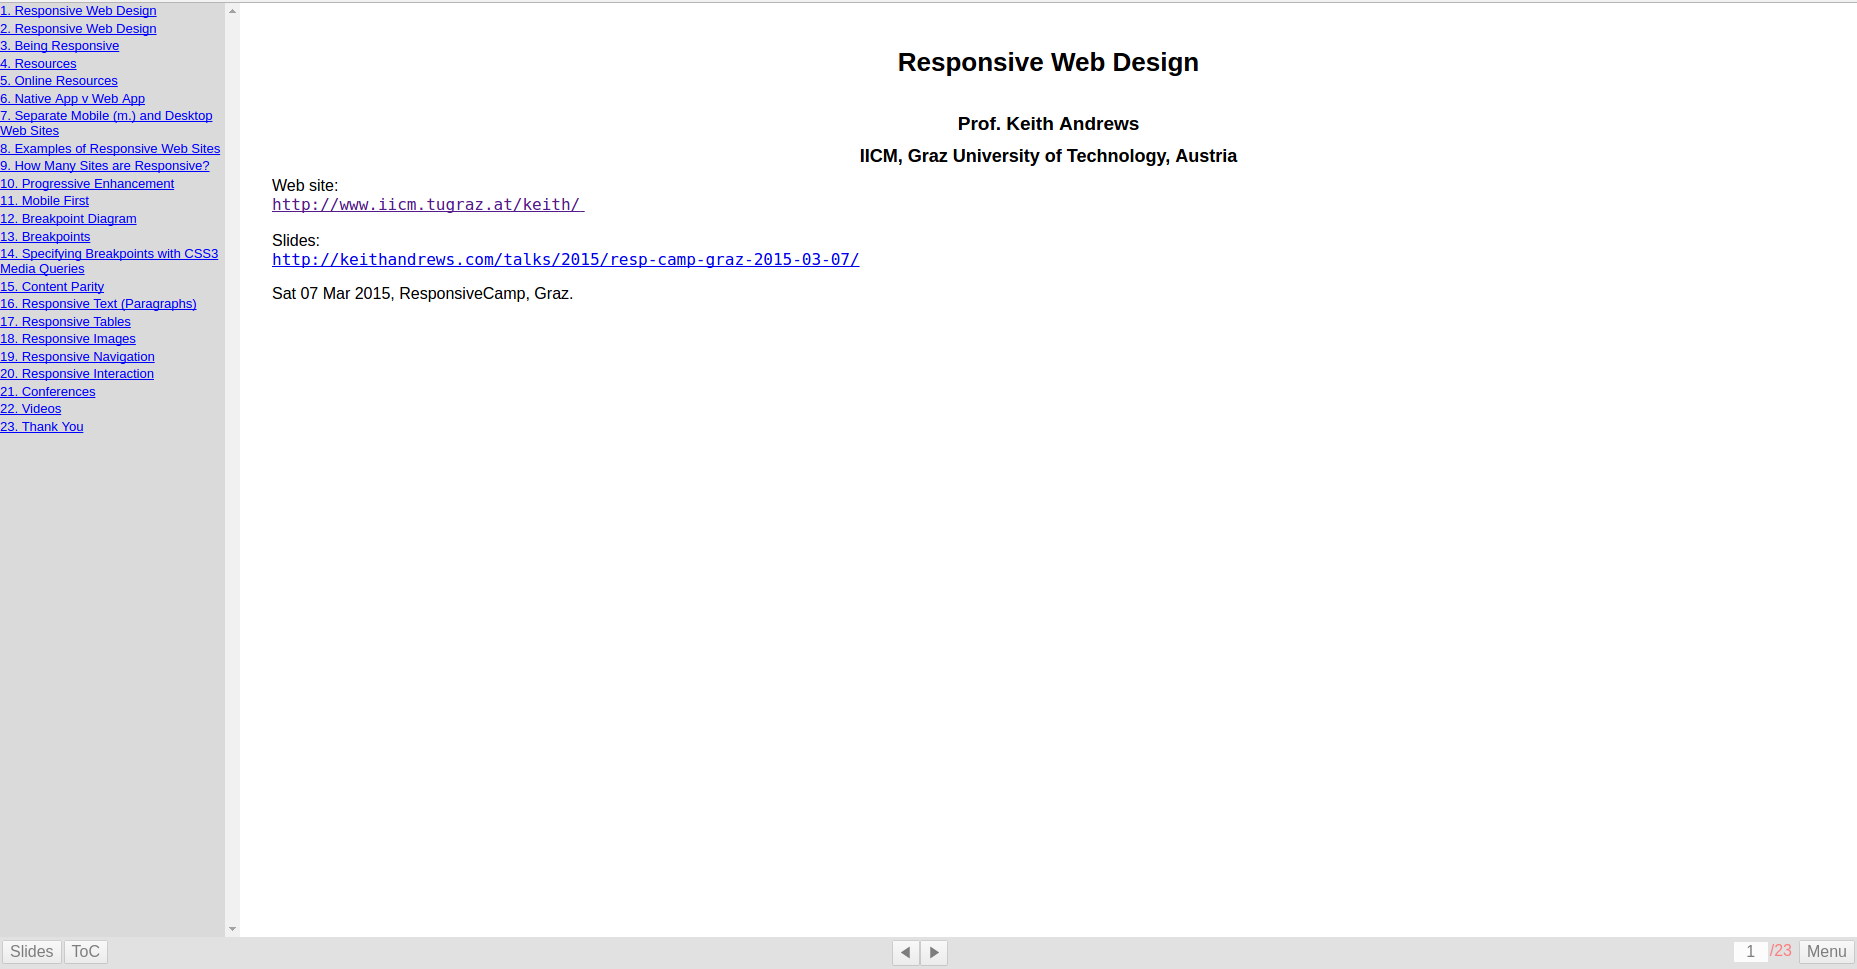
\includegraphics[width = .9\textwidth]{images/tocOld.png}
	
	\caption[Original Side Menus]{
		Design of \textit{rSlidy}'s original Slides and ToC side menus, 
both fixed and overlapped on left side of user interface.
		\imgcredit{Screenshot taken by the authors of this report.}
	}
	\label{fig:sideOLD}
\end{figure}
\begin{figure}[tp]
	\centering
	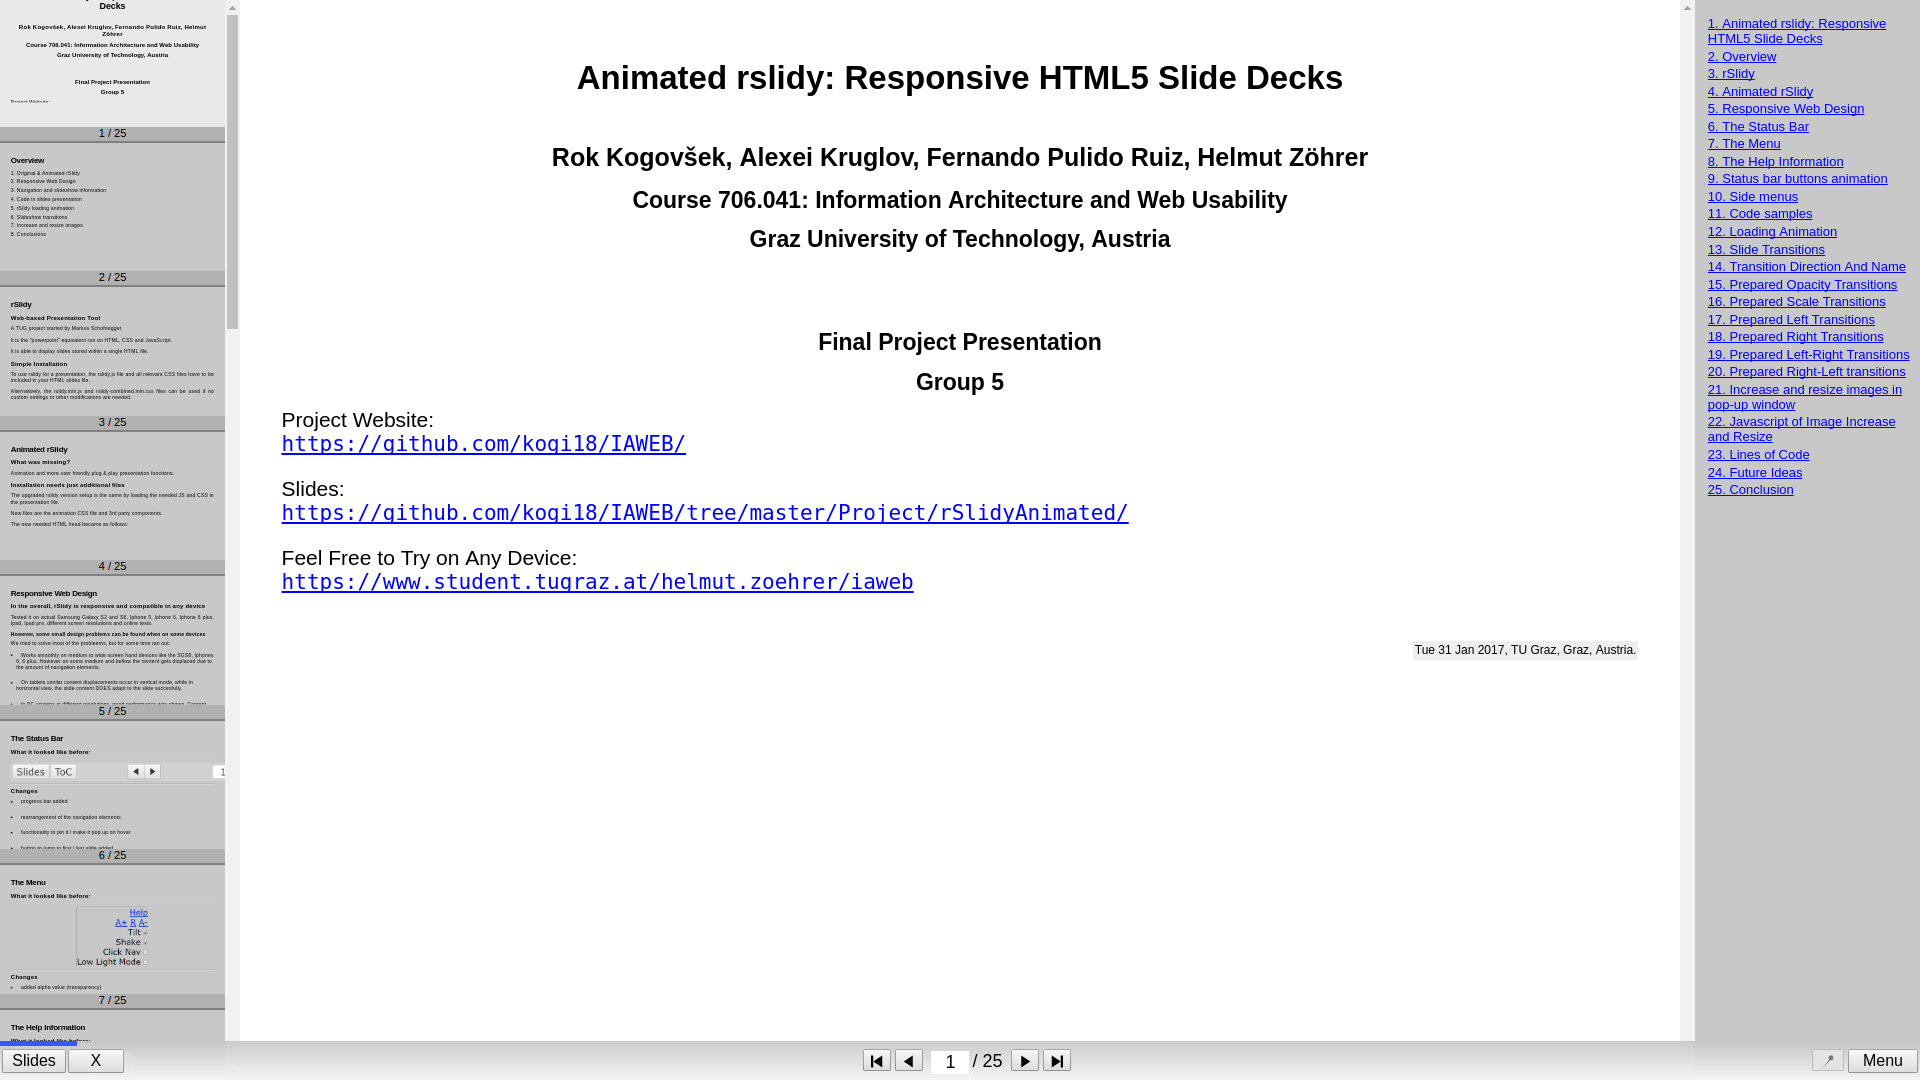
\includegraphics[width = .9\textwidth]{images/sidemenus.png}
	
	\caption[Modified Side Menus]{
		Design of \textit{rSlidy}'s modified Slides and ToC side menus, 
which open on hover and lock to the screen on button click. SLides overview is 
fixed to left side and ToC is fixed to the right side.
		\imgcredit{Screenshot taken by the authors of this report.}
	}
	\label{fig:sideNEW}
\end{figure}

% section side_menus (end)